\documentclass{article}

\usepackage{amsmath}
\usepackage{graphicx}
\usepackage{tikz}
\usepackage{pgfplots}
 
\begin{document}

\title{AI Coffe Club (09/01/2020)\\ Activation Functions}
\date{}

\maketitle

\begin{center}
Last modification: \today\\
\end{center}

Activation functions are used to modify or control the output of layers of a neural network. More precisely, they are applied to each neuron and they determine whether they should be activated or not and, in more complex cases, the magnitude of such activation.

Although activation functions were traditionally used as a mathematical gate, a simple step function, to turn the neuron on and off depending on a threshold to produce binary classifications, nowadays they are used for more complex purposes.

Modern neural networks use non-linear activation functions to create complex mappings between the inputs and the output and generate more complex decision boundaries to tackle difficult classification problems.

Many activation functions have been proposed to date, most of them trying to strike a balance between making the training easier, increasing representation capacity, avoiding common training stalemates, and computational efficiency. Table \ref{table:activations} shows a summarized overview.

\textbf{Remark: we need activation functions to be differentiable so as to perform backpropagation optimization.}

\begin{table}[!htb]
  \centering
  \resizebox{\linewidth}{!}{
  \begin{tabular}{|c|c|c|c|}
    \hline
    Name & Function & Derivative & Range\\
    \hline
    Sigmoid & $\sigma(x) = \frac{1}{1 + e^{-x}}$ & $\sigma'(x) = \sigma(x)(1 - \sigma(x))$ & $(0,1)$\\
    \hline
    Hyperbolic Tangent & $\sigma(x) = \frac{e^{2x} -1}{e^{2x} + 1}$ & $\sigma'(x) = 1 - \sigma(x)^2$ & $(-1,1)$\\
    \hline
    ReLU & $\sigma(x) =
    \begin{cases}
      0 & x \leq 0\\
      x & x > 0
    \end{cases}$ & $\sigma(x) =
    \begin{cases}
      0 & x \leq 0\\
      x & x > 0
    \end{cases}$ & $[0, \infty)$\\
    \hline
    Leaky ReLU & $\sigma(x) =
    \begin{cases}
      0.01x & x \leq 0\\
      x & x > 0
    \end{cases}$ & $\sigma(x) =
    \begin{cases}
      0.01 & x \leq 0\\
      x & x > 0
    \end{cases}$ & $(-\infty, \infty)$\\
    \hline
    Parametric ReLU & $\sigma(x) =
    \begin{cases}
      \alpha x & x \leq 0\\
      x & x > 0
    \end{cases}$ & $\sigma(x) =
    \begin{cases}
      \alpha & x \leq 0\\
      x & x > 0
    \end{cases}$ & $(-\infty, \infty)$\\
    \hline
    ELU & $\sigma(x) =
    \begin{cases}
      \alpha(e^x -1) & x \leq 0\\
      x & x > 0
    \end{cases}$ & $\sigma(x) =
    \begin{cases}
      \alpha + \sigma(x) & x \leq 0\\
      x & x > 0
    \end{cases}$ & $(-\alpha, \infty)$\\
    \hline
    Softplus & $\sigma(x) = \ln(1 + e^x)$ & $\sigma'(x) = \frac{1}{1 + e^{-x}}$ & $(0, \infty)$\\
    \hline
    Swish & $\sigma(x) = \frac{x}{1 + e^{-\beta x}}$ & $\sigma'(x) = \beta\sigma(x) + \frac{1}{1 + e^{-\beta x}}(1 - \beta\sigma(x))$ & \\
    \hline
  \end{tabular}}
  \caption{Common activation functions.}
  \label{table:activations}
\end{table}

\clearpage

\section{Sigmoid}

\begin{figure}[!htb]
  \centering
  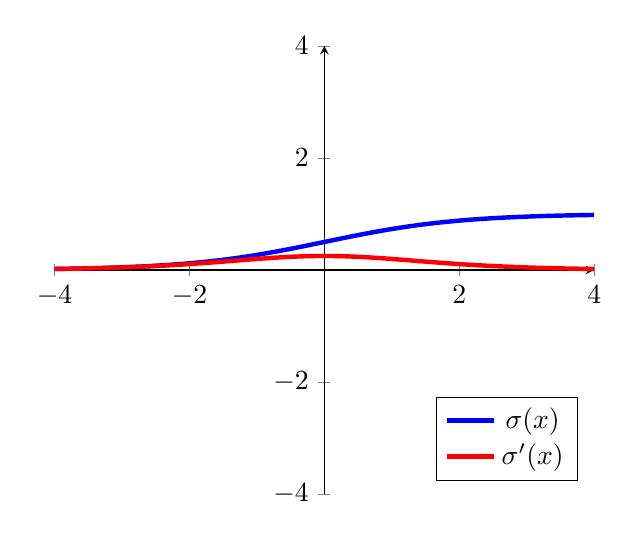
\begin{tikzpicture}
    \begin{axis}[
      axis lines= middle,
      legend pos= south east,
      xmax=4,
      xmin=-4,
      ymin=-4,
      ymax=4,
      samples=100]
      \addplot[blue, ultra thick]{(1 / (1 + e^(-x)))};
      \addplot[red, ultra thick]{((1 / (1 + e^(-x))) * (1.0 - (1 / (1 + e^(-x)))))};
      \legend{$\sigma(x)$, $\sigma'(x)$}
    \end{axis}
  \end{tikzpicture}
\end{figure}

\begin{equation}
\sigma(x) = \frac{1}{1 + e^{-x}}
\end{equation}

\begin{equation}
\sigma'(x) = \sigma(x)(1 - \sigma(x))
\end{equation}

\clearpage

\section{Hyperbolic Tangent}

\begin{figure}[!htb]
  \centering
  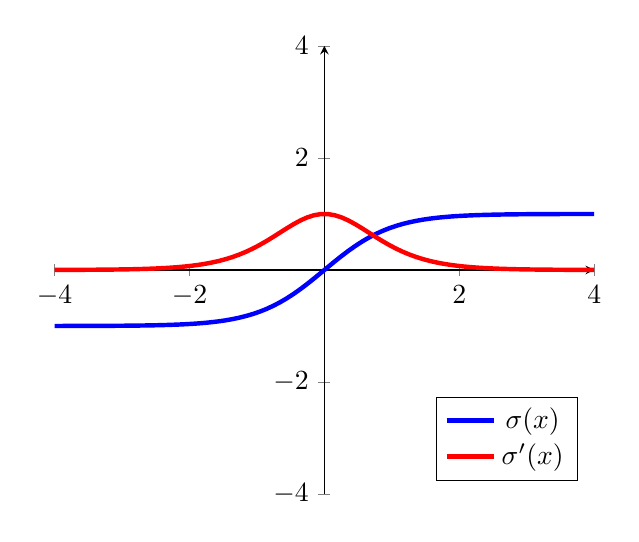
\begin{tikzpicture}
    \begin{axis}[
      axis lines= middle,
      legend pos= south east,
      xmax=4,
      xmin=-4,
      ymin=-4,
      ymax=4,
      samples=100]
      \addplot[blue, ultra thick]{(tanh(x))};
      \addplot[red, ultra thick]{( 1 - tanh(x)^2)};
      \legend{$\sigma(x)$, $\sigma'(x)$}
    \end{axis}
  \end{tikzpicture}
\end{figure}

\begin{equation}
\sigma(x) = tanh(x) = \frac{e^x - e^{-x}}{e^x + e^{-x}} = \frac{e^{2x} -1}{e^{2x} + 1}
\end{equation}

\begin{equation}
\sigma'(x) = 1 - \sigma(x)^2
\end{equation}

\clearpage

\section{Rectified Linear Unit}

\begin{equation}
\sigma(x) =
  \begin{cases}
    0 & x \leq 0\\
    x & x > 0
  \end{cases}
\end{equation}

\begin{equation}
\sigma'(x) =
  \begin{cases}
    0 & x \leq 0\\
    1 & x > 0
  \end{cases}
\end{equation}

\clearpage

\section{Leaky Rectified Linear Unit}

\begin{equation}
  \sigma(x) =
    \begin{cases}
      0.01x & x \leq 0\\
      x & x > 0
    \end{cases}
\end{equation}
  
\begin{equation}
  \sigma'(x) =
    \begin{cases}
      0.01 & x \leq 0\\
      1 & x > 0
    \end{cases}
\end{equation}

\clearpage

\section{Parametric Rectified Linear Unit}

\begin{equation}
  \sigma(x) =
    \begin{cases}
      \alpha x & x \leq 0\\
      x & x > 0
    \end{cases}
\end{equation}

\begin{equation}
  \sigma'(x) =
    \begin{cases}
      \alpha & x \leq 0\\
      1 & x > 0
    \end{cases}
\end{equation}

\clearpage

\section{Exponential Linear Unit}

\begin{equation}
  \sigma(x) =
    \begin{cases}
      \alpha(e^x - 1) & x \leq 0\\
      x & x > 0
    \end{cases}
\end{equation}

\begin{equation}
  \sigma'(x) =
    \begin{cases}
      \alpha + \sigma(x) & x \leq 0\\
      1 & x > 0
    \end{cases}
\end{equation}

\clearpage

\section{Softplus}

\begin{figure}[!htb]
  \centering
  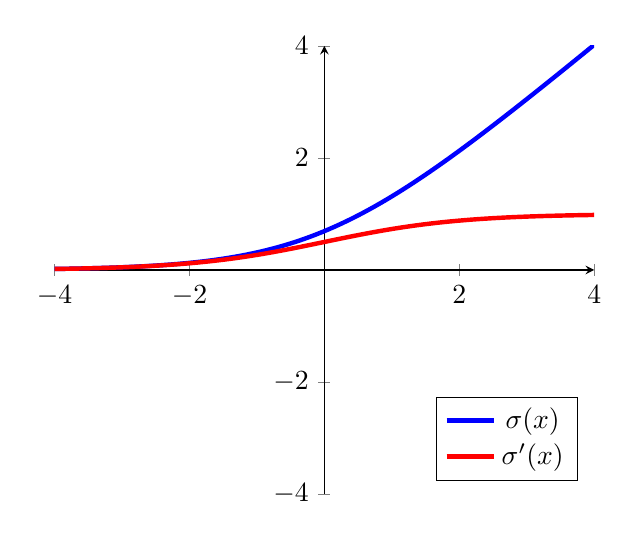
\begin{tikzpicture}
    \begin{axis}[
      axis lines= middle,
      legend pos= south east,
      xmax=4,
      xmin=-4,
      ymin=-4,
      ymax=4,
      samples=100]
      \addplot[blue, ultra thick]{(ln(1 + e^x))};
      \addplot[red, ultra thick]{(1.0 / (1 + e^(-x)))};
      \legend{$\sigma(x)$, $\sigma'(x)$}
    \end{axis}
  \end{tikzpicture}
\end{figure}

\begin{equation}
  \sigma(x) = \ln(1 + e^x)
\end{equation}

\begin{equation}
  \sigma'(x) = \frac{1}{1 + e^{-x}}
\end{equation}

\clearpage

\section{Swish}

\begin{figure}[!htb]
  \centering
  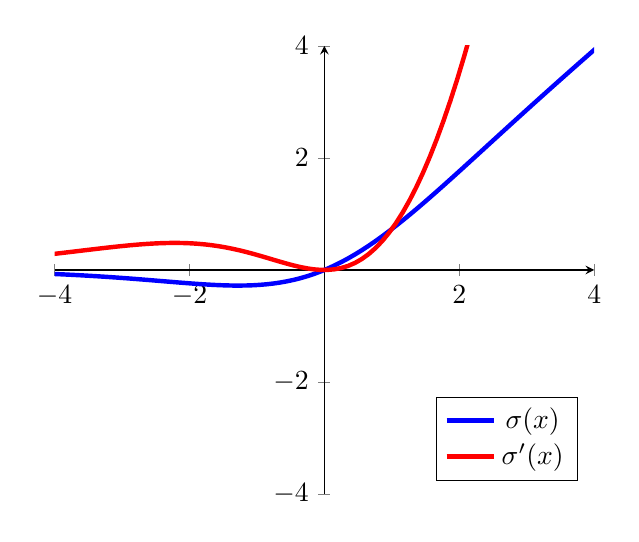
\begin{tikzpicture}
    \begin{axis}[
      axis lines= middle,
      legend pos= south east,
      xmax=4,
      xmin=-4,
      ymin=-4,
      ymax=4,
      samples=100]
      \addplot[blue, ultra thick]{(x / (1 + e^(-x)))};
      \addplot[red, ultra thick]{(x * (x / (1 + e^(-x))))};
      \legend{$\sigma(x)$, $\sigma'(x)$}
    \end{axis}
  \end{tikzpicture}
\end{figure}

\begin{equation}
\sigma(x) = \frac{x}{1 + e^{-x}}
\end{equation}

\begin{equation}
\sigma'(x) = x\sigma(x)
\end{equation}

\end{document}